% Provenance (never printed): old seconde/premiere S material on the
% atmosphere (storms, cyclones, the energy of the water cycle) and the
% natural-hazard themes of SVT; see sources/book2/PROVENANCE.md. Tracks,
% genesis statistics and the pressure--wind relation are computed in
% figdata/grade-10/cyclones.py from IBTrACS v04r01; the surge, thunder and
% energy numbers in the same script.
\chapter{Onweer en tropische cyclonen}\label{ch:g10:storms-and-cyclones}

Een hete zomermiddag eindigt in onweer. De lucht wordt donker, een windvlaag
koude lucht veegt door de straat, een flits verlicht de wolken --- en je begint
te tellen: een, twee, drie, \ldots{} negen seconden later rolt de donder. Het
onweer is ongeveer drie kilometer ver. Over een uur is het voorbij, en is de
lucht koel en schoon. Boven de warme tropische oceanen kunnen dezelfde
ingrediënten --- warme, vochtige lucht die opstijgt en condenseert --- zich
organiseren tot stormen van een heel andere orde: tropische cyclonen, honderden
kilometers breed, die dagen duren en winden brengen die sterk genoeg zijn om
bossen plat te leggen, en een stijging van de zee die hele kusten overstroomt.
Dit hoofdstuk bekijkt \omterm{def:g10:storms-and-cyclones:thunderstorm}{onweersbuien}, \omterm{def:g10:storms-and-cyclones:tornado}{tornado}'s en tropische cyclonen, en waar hun
energie vandaan komt.

\begin{safety}
Als je de donder kunt horen, kan de \omterm{def:g10:storms-and-cyclones:lightning}{bliksem} je bereiken. Ga een gebouw of een
gesloten auto in en blijf daar tot ruim na de laatste donderslag. Schuil nooit
onder een alleenstaande boom, en blijf weg van heuveltoppen, open velden en water.
\end{safety}

\begin{recall}
Luchtmassa's, fronten, depressies (gebieden met lage luchtdruk) en
anticyclonen worden op weerkaarten getekend met isobaren, lijnen van gelijke
druk (Boek 1, jaar 8). Een natuurgevaar is een natuurlijke gebeurtenis die
mensen en wat ze bouwen schade kan toebrengen (Boek 1, jaar 5). Geluid plant
zich in lucht voort met ongeveer \qty{340}{m/s}, licht bijna ogenblikkelijk (de
natuurkundeboeken). Warme, vochtige lucht die opstijgt, koelt af, condenseert op
haar \omterm{def:g10:why-clouds-form:condensation-level}{condensatieniveau} tot wolken en geeft \omterm{def:g10:earth-energy-budget:latent-heat}{latente warmte} af; verzadigde lucht
is vaak onstabiel (\cref{ch:g10:why-clouds-form}).
\end{recall}

\section{Onweersbuien}

\begin{definition}[Onweersbui]\label{def:g10:storms-and-cyclones:thunderstorm}
Een \emph{onweersbui}\index{onweersbui} is een bui die door een
cumulonimbuswolk wordt veroorzaakt, met \omterm{def:g10:storms-and-cyclones:lightning}{bliksem} en donder, meestal met zware
regenbuien en windstoten, soms met hagel.
\end{definition}

Een \omterm{def:g10:storms-and-cyclones:thunderstorm}{onweersbui} groeit uit onstabiele, vochtige lucht. In het eerste stadium
groeit een cumulus omhoog, gevoed door een sterke opwaartse luchtstroom;
condensatie geeft \omterm{def:g10:earth-energy-budget:latent-heat}{latente warmte} af en houdt de stijgende lucht warmer dan haar
omgeving. In het rijpe stadium bereikt de wolk de \omterm{def:g10:why-clouds-form:stability}{stabiele lucht} hoog erboven en
spreidt ze zich uit tot een aambeeld; druppels en hagelstenen worden groot genoeg
om te vallen, en de vallende regen sleurt koude lucht mee naar beneden: een
neerwaartse luchtstroom die zich aan de grond uitspreidt als een koud
windstootfront. In het laatste stadium neemt de neerwaartse stroom de hele wolk
over, waardoor de aanvoer van warme, vochtige lucht wordt afgesneden, en het
onweer regent zichzelf uit.

\begin{omfigure}
\begin{tikzpicture}[font=\footnotesize, >={Stealth[length=2mm]}]
  \foreach \dx/\title in {0/{1. groeistadium}, 4.6/{2. rijp stadium}, 9.2/{3. uitdoving}}
    \node[anchor=north] at (\dx+1.6,-0.15) {\title};
  \draw[thick, black!60] (-0.3,0) -- (12.9,0);
  % stage 1: a tall cumulus
  \pic[scale=1.4, transform shape] at (1.6,1.2) {puffycloud};
  \pic[scale=1.1, transform shape] at (1.6,2.0) {puffycloud};
  \foreach \x in {1.2,1.6,2.0} \draw[->, thick, omThm!80!black] (\x,0.2) -- (\x,2.6);
  % stage 2: cumulonimbus with anvil
  \fill[black!8, draw=black!50] (5.0,1.0) -- (4.9,4.0) -- (4.2,4.4) -- (8.0,4.6) -- (7.4,4.0) -- (7.2,1.0) -- cycle;
  \draw[->, thick, omThm!80!black] (5.5,0.2) -- (5.5,4.2);
  \draw[->, thick, omThm!80!black] (5.9,0.2) -- (5.9,4.2);
  \draw[->, thick, omDef!80!black] (6.7,3.4) -- (6.7,0.3) -- (7.6,0.3);
  \foreach \x in {6.4,6.85,7.05} \draw[omDef!50] (\x,0.95) -- (\x-0.1,0.1);
  \node[anchor=west, align=left] at (8.0,4.6) {aambeeld};
  \node[anchor=west, align=left, omDef!80!black] at (7.65,0.45) {windstootfront};
  % stage 3: dissipating
  \fill[black!8, draw=black!50] (9.7,1.2) -- (9.6,3.6) -- (9.0,4.0) -- (12.6,4.1) -- (12.0,3.6) -- (11.8,1.2) -- cycle;
  \foreach \x in {10.3,10.9,11.5} \draw[->, thick, omDef!80!black] (\x,3.2) -- (\x,0.3);
  \foreach \x in {10.6,11.2} \draw[omDef!50] (\x,1.15) -- (\x-0.1,0.1);
  % legend
  \draw[->, thick, omThm!80!black] (0,5.0) -- (0,5.5); \node[anchor=west] at (0.1,5.25) {warme opwaartse stroom};
  \draw[->, thick, omDef!80!black] (3.2,5.5) -- (3.2,5.0); \node[anchor=west] at (3.3,5.25) {koude neerwaartse stroom};
\end{tikzpicture}

{\small De drie stadia van een \omterm{def:g10:storms-and-cyclones:thunderstorm}{onweersbui} (schematisch, niet op schaal): een
groeiende cumulus, gevoed door opwaartse stromen; de rijpe cumulonimbus, met
zijn aambeeld, zijn opwaartse stroom en een neerwaartse stroom die door de regen
wordt meegesleurd; het uitdovende onweer, één en al neerwaartse stroom.}
\end{omfigure}

In de wolk scheiden botsingen tussen ijsdeeltjes, die door de lucht op en neer
worden gevoerd, elektrische ladingen: de wolk raakt geladen, meestal negatief
aan de onderkant en positief aan de bovenkant, en de grond eronder krijgt een
eigen lading.

\begin{definition}[Bliksem]\label{def:g10:storms-and-cyclones:lightning}
\emph{Bliksem}\index{bliksem} is een reusachtige elektrische vonk die geladen
gebieden van een \omterm{def:g10:storms-and-cyclones:thunderstorm}{onweersbui} ontlaadt, in de wolk, tussen wolken, of tussen de
wolk en de grond. Hij verhit een smal luchtkanaal zo plotseling dat de lucht met
een schok uitzet: het geluid van die uitzetting is de \emph{donder}.
\end{definition}

\begin{omfigure}
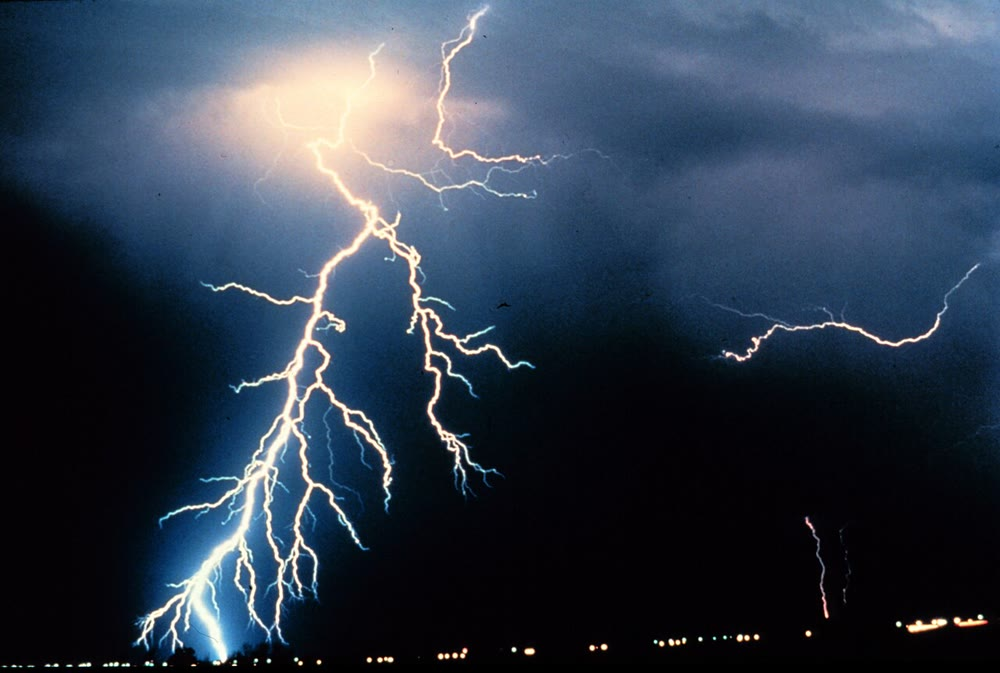
\includegraphics[width=0.62\linewidth]{images/book2/g10-noaa-lightning.jpg}

{\small Bliksemontladingen, tussen wolken en van de wolk naar de grond, tijdens
een nachtelijk onweer. Foto: C.~Clark, NOAA National Severe Storms Laboratory
(publiek domein).}
\end{omfigure}

Satellieten die de lichtflitsen over de hele planeet tellen, vinden ongeveer
1.4 miljard bliksemflitsen per jaar, of 44 per seconde.
% ledger: christian:flash-rate

\begin{method}[De afstand van een onweer uit flits en donder]\label{met:g10:storms-and-cyclones:distance}
\begin{enumerate}
  \item Het licht van de flits komt praktisch meteen aan; de donder plant zich
        voort met de geluidssnelheid, ongeveer \qty{343}{m/s} bij
        \qty{20}{\degreeCelsius}.
  \item Tel het aantal seconden $t$ tussen de flits en de donder.
  \item De afstand is $343\,t$ meter: ongeveer \qty{1}{km} per drie
        seconden.
\end{enumerate}
\end{method}
% ledger: const:R, earth:Mmol (speed of sound computed in figdata/grade-10/cyclones.py)

\section{Tornado's}

\begin{definition}[Tornado]\label{def:g10:storms-and-cyclones:tornado}
Een \emph{tornado}\index{tornado} is een hevig draaiende luchtkolom die contact
maakt met de grond en aan de onderkant van een cumulonimbus hangt.
\end{definition}

De sterkste \omterm{def:g10:storms-and-cyclones:tornado}{tornado}'s komen uit \emph{supercellen}, \omterm{def:g10:storms-and-cyclones:thunderstorm}{onweersbuien} waarvan de
opwaartse stroom als geheel draait. Een \omterm{def:g10:storms-and-cyclones:tornado}{tornado} is klein en kortstondig:
meestal een paar honderd meter breed, enkele minuten lang, met een gemiddeld
spoor van ongeveer \qty{5.6}{km}. Maar zijn winden zijn de sterkste aan het
aardoppervlak: een mobiele radar mat in mei 1999 in een \omterm{def:g10:storms-and-cyclones:tornado}{tornado} in Oklahoma
ongeveer \qty{135}{m/s} (zo'n \qty{480}{km/h}) boven de grond. De Verenigde
Staten hebben meer \omterm{def:g10:storms-and-cyclones:tornado}{tornado}'s dan enig ander land, rond de 1200 per jaar; andere
gebieden waar ze vaak voorkomen, zijn onder meer de Canadese prairies,
Bangladesh, het noorden van Argentinië en het zuiden van Brazilië, en
Groot-Brittannië.
% ledger: spc:tornado

\begin{omfigure}
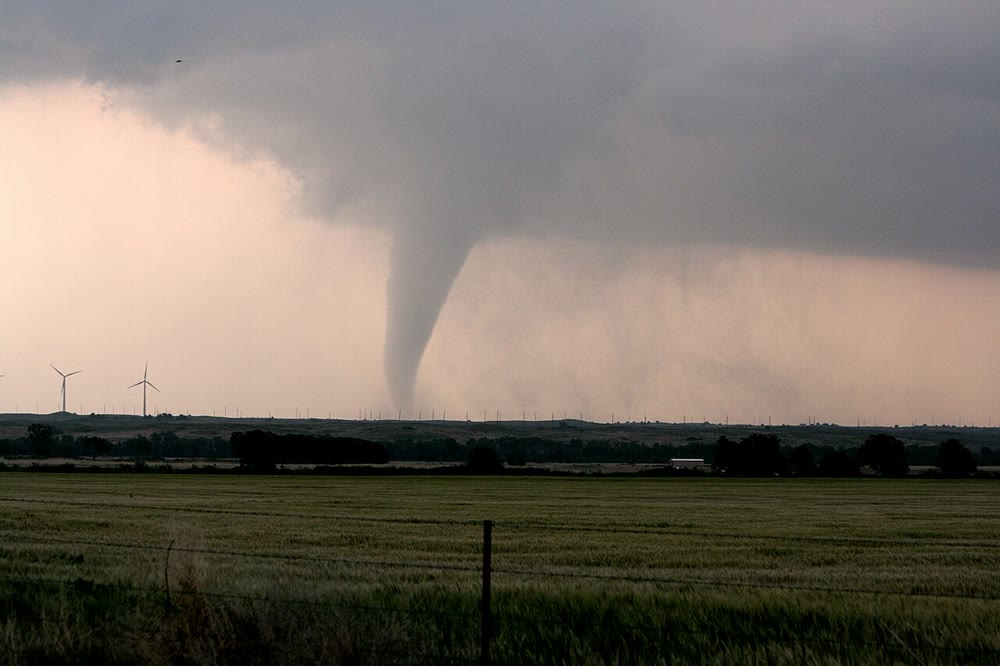
\includegraphics[width=0.62\linewidth]{images/book2/g10-noaa-tornado-kansas.jpg}

{\small Een \omterm{def:g10:storms-and-cyclones:tornado}{tornado} boven de vlakten van Kansas, mei 2008: de slurf hangt aan de
onderkant van de onweerswolk. Foto: Sean Waugh, NOAA National Severe Storms
Laboratory (publiek domein).}
\end{omfigure}

\section{Tropische cyclonen}

\begin{definition}[Tropische cycloon; oog; oogwand]\label{def:g10:storms-and-cyclones:tropical-cyclone}
Een \emph{tropische cycloon}\index{tropische cycloon} is een storm van honderden
kilometers breed die boven een warme tropische zee ontstaat rond een centrum van
lage druk, met winden die in een spiraal naar het centrum toe draaien en banden
van \omterm{def:g10:storms-and-cyclones:thunderstorm}{onweersbuien}. Als zijn aanhoudende wind \num{64}~knopen bereikt, ongeveer
\qty{119}{km/h}, heet hij een orkaan in de Atlantische Oceaan en het oosten van
de Grote Oceaan, een tyfoon in het westen van de Grote Oceaan, en gewoon een
cycloon in de Indische Oceaan en de zuidelijke Grote Oceaan. Zijn rustige,
bijna wolkeloze centrum is het \emph{oog}\index{oog}; de ring van torenhoge
\omterm{def:g10:storms-and-cyclones:thunderstorm}{onweersbuien} eromheen, waar de wind het sterkst is, is de
\emph{oogwand}\index{oogwand}.
\end{definition}
% ledger: nhc:sshws

\begin{omfigure}
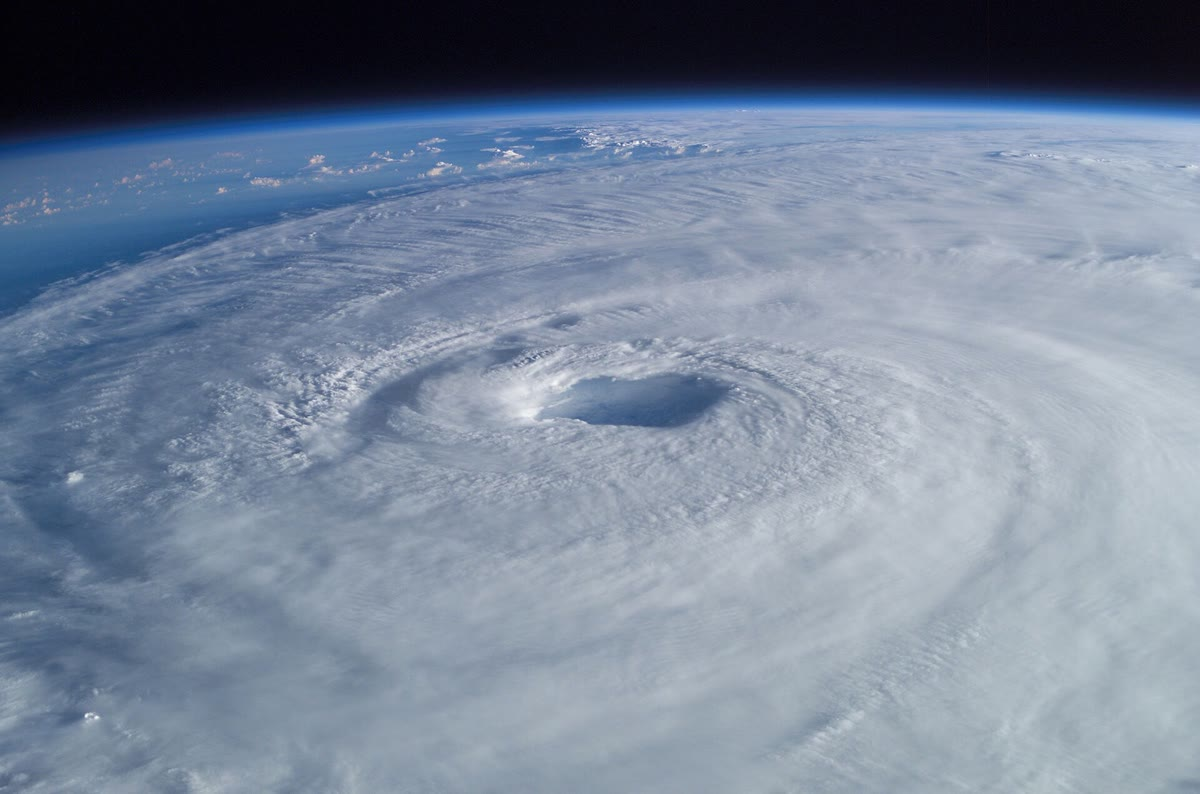
\includegraphics[width=0.78\linewidth]{images/book2/g10-nasa-hurricane-isabel.jpg}

{\small Orkaan Isabel, 15 september 2003, gefotografeerd door een astronaut
vanuit het Internationaal Ruimtestation: het \omterm{def:g10:storms-and-cyclones:tropical-cyclone}{oog}, de \omterm{def:g10:storms-and-cyclones:tropical-cyclone}{oogwand} en de spiraal van
wolken eromheen. Beeld: Mike Trenchard, Earth Sciences and Image Analysis
Laboratory, NASA Johnson Space Center (publiek domein).}
\end{omfigure}

Vlak boven het zeeoppervlak stroomt vochtige lucht naar de lage druk van het
centrum. De draaiing van de Aarde buigt bewegende lucht op het noordelijk
halfrond naar rechts af: in plaats van recht naar het centrum te gaan, draait
de lucht eromheen, tegen de wijzers van de klok in van bovenaf gezien (met de
klok mee op het zuidelijk halfrond). Dicht bij het centrum stijgt ze op in de
\omterm{def:g10:storms-and-cyclones:tropical-cyclone}{oogwand}, condenseert, en stroomt bovenaan de storm weg. In het \omterm{def:g10:storms-and-cyclones:tropical-cyclone}{oog} daalt een
beetje lucht, die opwarmt en opdroogt: de lucht klaart op.

\begin{omfigure}
\begin{tikzpicture}[font=\footnotesize, >={Stealth[length=2mm]}]
  \fill[omDef!25] (-6,-0.4) rectangle (6,0);
  \node[anchor=north, omDef!80!black] at (0,-0.05) {warme zee};
  % rain bands
  \foreach \x/\h in {-5.0/1.6, -3.9/2.2, 3.9/2.2, 5.0/1.6}
    \fill[black!10, draw=black!45] (\x-0.35,0.4) -- (\x-0.3,\h) .. controls (\x-0.15,\h+0.35) and (\x+0.15,\h+0.35) .. (\x+0.3,\h) -- (\x+0.35,0.4) -- cycle;
  % eyewall towers and outflow canopy
  \fill[black!14, draw=black!50] (-2.4,0.4) -- (-2.5,4.0) -- (-5.8,4.3) -- (-5.6,4.7) -- (-1.0,4.9) -- (-0.75,4.0) -- (-0.8,0.4) -- cycle;
  \fill[black!14, draw=black!50] (2.4,0.4) -- (2.5,4.0) -- (5.8,4.3) -- (5.6,4.7) -- (1.0,4.9) -- (0.75,4.0) -- (0.8,0.4) -- cycle;
  % inflow, rise, outflow, eye subsidence
  \draw[->, thick, omThm!80!black] (-5.8,0.2) -- (-1.3,0.2) -- (-1.3,4.3) -- (-4.2,4.45);
  \draw[->, thick, omThm!80!black] (5.8,0.2) -- (1.3,0.2) -- (1.3,4.3) -- (4.2,4.45);
  \draw[->, thick, omDef!80!black] (0,4.3) -- (0,1.0);
  \node[anchor=south, align=center] at (0,5.0) {oog: dalende\\droge lucht};
  \node[anchor=south east, align=right] at (-2.6,4.95) {oogwand};
  \node[anchor=west, align=left] at (-5.95,2.9) {regen-\\banden};
  \node[anchor=north, align=center] at (-3.6,0.15) {vochtige instroom};
  \node[anchor=south east, align=right] at (5.8,4.95) {uitstroom in de hoogte};
  % plan view
  \begin{scope}[shift={(8.4,2.3)}]
    \draw[black!40] (0,0) circle (1.7);
    \foreach \a in {0,90,180,270}
      \draw[->, thick, omThm!80!black, domain=0:200, samples=30, variable=\t]
        plot ({(1.6-0.0045*\t)*cos(\a+\t)}, {(1.6-0.0045*\t)*sin(\a+\t)});
    \fill[white, draw=black!50] (0,0) circle (0.22);
    \node[anchor=north, align=center] at (0,-1.8) {van bovenaf gezien\\(noordelijk halfrond)};
  \end{scope}
\end{tikzpicture}

{\small Een \omterm{def:g10:storms-and-cyclones:tropical-cyclone}{tropische cycloon} in doorsnede (schematisch, hoogte sterk
overdreven): vochtige lucht stroomt boven de warme zee naar binnen, stijgt op in
de \omterm{def:g10:storms-and-cyclones:tropical-cyclone}{oogwand} en de regenbanden, en stroomt bovenaan weg; in het \omterm{def:g10:storms-and-cyclones:tropical-cyclone}{oog} daalt een
beetje lucht. Rechts: van bovenaf gezien op het noordelijk halfrond draait de
instroom tegen de wijzers van de klok in rond het centrum.}
\end{omfigure}

Tropische cyclonen hebben een warme oceaan nodig: water van minstens ongeveer
\qty{27}{\degreeCelsius} aan het oppervlak, warm tot op een diepte van zo'n
\qty{46}{m}. Ze ontstaan niet op de evenaar zelf, waar de draaiing van de Aarde
de instromende lucht geen draai geeft: een storm moet minstens ongeveer
\qty{480}{km} van de evenaar liggen om te gaan draaien.
% ledger: aoml:formation

\begin{omfigure}
\begin{tikzpicture}
\begin{axis}[ommap, width=\linewidth, xtick={-180,-120,...,180}, ytick={-60,-30,0,30,60},
  ymin=-70, ymax=70, unbounded coords=jump]
\addplot[fill=omLithAlluv, draw=black!45, line width=0.2pt] table {figdata/out/shared-geo-land.dat};
\addplot[omThm!70, line width=0.25pt] table {figdata/out/grade-10-cyclones-tracks.dat};
\addplot[only marks, mark=*, mark size=0.45pt, omDef!90!black] table {figdata/out/grade-10-cyclones-genesis.dat};
\addplot[black!45, dashed, domain=-180:180] {0};
\end{axis}
\end{tikzpicture}

{\small Tropische cyclonen: de banen van alle stormen van de seizoenen
2015--2024 (rood), en de plaats waar elke storm van de seizoenen 1980--2024 voor
het eerst de kracht van een tropische storm bereikte (blauwe stippen).
Gegevens: IBTrACS v04r01, NOAA National Centers for Environmental Information.}
\end{omfigure}
% ledger: data:b2-ibtracs (all statistics computed in figdata/grade-10/cyclones.py)

De kaart toont de regel aan het werk. Van de 3\,888 stormen van 1980--2024
bereikten er maar 24 de kracht van een tropische storm binnen \qty{5}{\degree}
van de evenaar. De meeste ontstaan tussen \qty{10}{\degree} en \qty{30}{\degree}
breedte, drijven dan met de passaatwinden naar het westen en buigen af naar de
polen, waar de koude zee ze verzwakt. De zuidelijke Atlantische Oceaan, koeler
en minder gunstig, zag er in 45 jaar maar drie. In een gemiddeld jaar ontstaan
er ongeveer 87 tropische cyclonen, zeven op de tien op het noordelijk halfrond,
en iets meer dan de helft bereikt orkaankracht.

\begin{proposition}[De energiebron van een tropische cycloon]\label{prop:g10:storms-and-cyclones:energy}
Een \omterm{def:g10:storms-and-cyclones:tropical-cyclone}{tropische cycloon} haalt zijn energie uit de warme zee: de \omterm{def:g10:earth-energy-budget:latent-heat}{latente warmte} die
bij verdamping aan het zeeoppervlak wordt opgenomen, komt in de \omterm{def:g10:storms-and-cyclones:tropical-cyclone}{oogwand} en de
regenbanden vrij wanneer de damp condenseert. Een gemiddelde orkaan maakt zo
ongeveer \qty{6e14}{W} vrij; maar een klein deel daarvan, ongeveer
\qty{1.5e12}{W}, gaat naar de bewegingsenergie van zijn winden.
\end{proposition}
% ledger: aoml:energy

\begin{proof}[Verantwoording]
Een gemiddelde orkaan laat per dag \qty{1.5}{cm} regen vallen over een cirkel
met straal \qty{665}{km}, een oppervlakte van $\pi \times (665\,000)^2 \approx
\qty{1.39e12}{m^2}$: \qty{2.1e10}{m^3}, of \qty{2.1e13}{kg}, water per dag.
Elke kilogram die condenseert, geeft ongeveer \qty{2.5}{MJ} vrij: $2.1\times10^{13}
\times 2.5\times10^6 \approx \qty{5.2e19}{J}$ per dag, dat is
$5.2\times10^{19}/86\,400 \approx \qty{6.0e14}{W}$. Het vermogen van de winden is
een schatting uit gemeten windvelden, overgenomen uit dezelfde bron.
\end{proof}

De storm werkt als een motor: warmte die aan het warme zeeoppervlak wordt
opgenomen en hoog in de koude bovenlucht wordt afgestaan, terwijl een deel van
het verschil wordt omgezet in de beweging van de wind. Daarom verzwakt een
\omterm{def:g10:storms-and-cyclones:tropical-cyclone}{tropische cycloon} snel wanneer hij boven land of boven koud water komt: hij
verliest zijn aanvoer van verdampend water.

\section{Intensiteit, wind en stormopzet}

\begin{definition}[Schaal van Saffir--Simpson]\label{def:g10:storms-and-cyclones:scale}
De \emph{schaal van Saffir--Simpson}\index{schaal van Saffir--Simpson} deelt
orkanen in vijf categorieën in naar hun maximale aanhoudende wind; de
categorieën 3 tot en met 5 zijn \emph{zware} orkanen.
\end{definition}

\begin{center}
\small
\begin{tabular}{cccc}
\hline
categorie & knopen & \unit{m/s} & \unit{km/h} \\
\hline
1 & 64--82 & 33--42 & 119--153 \\
2 & 83--95 & 43--49 & 154--177 \\
3 & 96--112 & 49--58 & 178--208 \\
4 & 113--136 & 58--70 & 209--251 \\
5 & 137 of meer & 70 of meer & 252 of meer \\
\hline
\end{tabular}
\end{center}
% ledger: nhc:sshws (m/s converted with 1 knot = 1852/3600 m/s)

Hoe dieper de lage druk in het centrum, hoe sterker de winden die eromheen waaien:
het drukverschil tussen het centrum en de omgeving is wat de lucht naar binnen
drijft.

\begin{omfigure}
\begin{tikzpicture}
\begin{axis}[omrecord, width=0.86\linewidth, height=6.2cm, xmin=15, xmax=100,
  ymin=860, ymax=1015, xlabel={maximale aanhoudende wind (\unit{m/s})},
  ylabel={minimale druk in het centrum (\unit{hPa})},
  tick label style={font=\small}, label style={font=\small}]
\foreach \w in {32.92, 42.70, 49.39, 58.13, 70.48}
  \edef\temp{\noexpand\draw[black!55, densely dashed] (axis cs:\w,860) -- (axis cs:\w,1015);}\temp
\addplot[only marks, mark=*, mark size=0.6pt, omDef!80!black, opacity=0.6] table[x=wind_ms, y=pmin_hpa] {figdata/out/grade-10-cyclones-scatter.dat};
\addplot[omThm!85!black, thick] table[x=wind_ms, y=pmin_hpa] {figdata/out/grade-10-cyclones-fit.dat};
\node[font=\scriptsize, black!60] at (axis cs:37.8,1008) {1};
\node[font=\scriptsize, black!60] at (axis cs:46.0,1008) {2};
\node[font=\scriptsize, black!60] at (axis cs:53.8,1008) {3};
\node[font=\scriptsize, black!60] at (axis cs:64.3,1008) {4};
\node[font=\scriptsize, black!60] at (axis cs:76,1008) {5};
\end{axis}
\end{tikzpicture}

{\small Elke stip is één \omterm{def:g10:storms-and-cyclones:tropical-cyclone}{tropische cycloon} van de seizoenen 2000--2024: zijn
sterkste aanhoudende wind en zijn laagste druk in het centrum. De lijn is de
best passende rechte: ongeveer \qty{1.6}{hPa} lager voor elke meter per seconde
extra. Grijze stippellijnen: de grenzen van de categorieën van Saffir--Simpson
(bovenaan genummerd). Gegevens: IBTrACS v04r01, NOAA NCEI.}
\end{omfigure}
% ledger: data:b2-ibtracs, nhc:sshws (fit computed in figdata/grade-10/cyclones.py)

Het record van de stormen van 1980--2024 in het archief staat op naam van orkaan
Patricia, voor de Pacifische kust van Mexico in oktober 2015: een aanhoudende
wind van 185 knopen, ongeveer \qty{95}{m/s}, en een druk in het centrum van
\qty{872}{hPa}.
% ledger: data:b2-ibtracs

\begin{definition}[Stormopzet]\label{def:g10:storms-and-cyclones:storm-surge}
\emph{Stormopzet}\index{stormopzet} is de stijging van de zee boven haar normale
niveau, getij niet meegerekend, die door een storm wordt veroorzaakt: de wind
stuwt water op tegen de kust, en door de lage druk bolt de zee onder de storm op.
\end{definition}

\begin{proposition}[De drukbult]\label{prop:g10:storms-and-cyclones:bulge}
Onder een storm waarvan de druk in het centrum $\Delta p$ hectopascal lager is
dan die van de omgeving, stijgt de zee met ongeveer $\Delta p$ centimeter.
\end{proposition}

\begin{proof}
Diep onder het oppervlak moet de druk onder de storm en daarbuiten gelijk zijn,
anders zou het water gaan stromen. De lucht boven de storm weegt $\Delta p$
minder; een kolom zeewater met hoogte $h$ maakt dat goed als
$\rho g h = \Delta p$. Voor $\Delta p = \qty{1}{hPa} = \qty{100}{Pa}$, met
$\rho = \qty{1025}{kg/m^3}$ en $g = \qty{9.81}{m/s^2}$: $h = 100/(1025
\times 9.81) \approx \qty{0.0099}{m}$, ongeveer \qty{1}{cm}.
\end{proof}
% ledger: noaa:seawater-1025, nasa:aquarius-density, const:gn

Bij de meeste stormopzetten is de drukbult het kleinste deel: onder een druk in
het centrum van \qty{920}{hPa}, \qty{90}{hPa} lager dan de omgeving, is hij
ongeveer \qty{0.9}{m}. De wind doet de rest en duwt water naar de kust, vooral
boven een brede, ondiepe zeebodem. Valt een opzet van enkele meters samen met
hoogwater, dan kan hij lage kusten tot ver landinwaarts overstromen.

\begin{omfigure}
\begin{tikzpicture}[font=\footnotesize, >={Stealth[length=2mm]}]
  \def\surf{(0,0) .. controls (1.5,0) and (2.2,0.5) .. (3.0,0.5) .. controls (3.8,0.5) and (4.6,0.4) .. (5.6,0.5) .. controls (7.2,0.65) and (8.8,1.0) .. (10.25,1.3)}
  \fill[omDef!20] (0,-1.6) -- \surf -- (8.8,-1.6) -- cycle;
  \draw[thick, omDef!80!black] \surf;
  \draw[black!50, dashed] (0,0) -- (9.6,0);
  \node[anchor=north west, black!60] at (0.1,-0.05) {normaal zeeniveau};
  \fill[omExo!30, draw=black!60] (8.8,-1.6) -- (10.4,1.6) -- (12.4,1.7) -- (12.4,-1.6) -- cycle;
  \foreach \x in {10.9,11.7} \draw[fill=white, draw=black!60] (\x,1.63) rectangle (\x+0.45,2.03) (\x-0.05,2.03) -- (\x+0.225,2.28) -- (\x+0.5,2.03);
  \draw[<->, omThm!80!black] (3.0,0) -- (3.0,0.5);
  \node[anchor=south east, omThm!80!black, align=right] at (2.8,0.6) {bult onder\\de lage druk};
  \draw[<->, omThm!80!black] (9.4,0) -- (9.4,1.12);
  \node[anchor=south, omThm!80!black, align=center] at (8.9,1.75) {windopzet\\tegen de kust};
  \foreach \y in {2.9,3.4} \draw[->, thick, black!60] (4.0,\y) -- (6.4,\y);
  \node[anchor=south] at (5.2,3.45) {aanlandige wind};
  \node[anchor=south, align=center] at (3.0,1.9) {centrum van\\de storm};
  \draw[black!40] (3.0,1.9) -- (3.0,0.65);
\end{tikzpicture}

{\small \omterm{def:g10:storms-and-cyclones:storm-surge}{Stormopzet} (schematisch, hoogten sterk overdreven): de zee stijgt met
ongeveer \qty{1}{cm} per hectopascal lage druk onder de storm, en de
aanlandige wind stuwt water op tegen de kust.}
\end{omfigure}

\begin{omfigure}
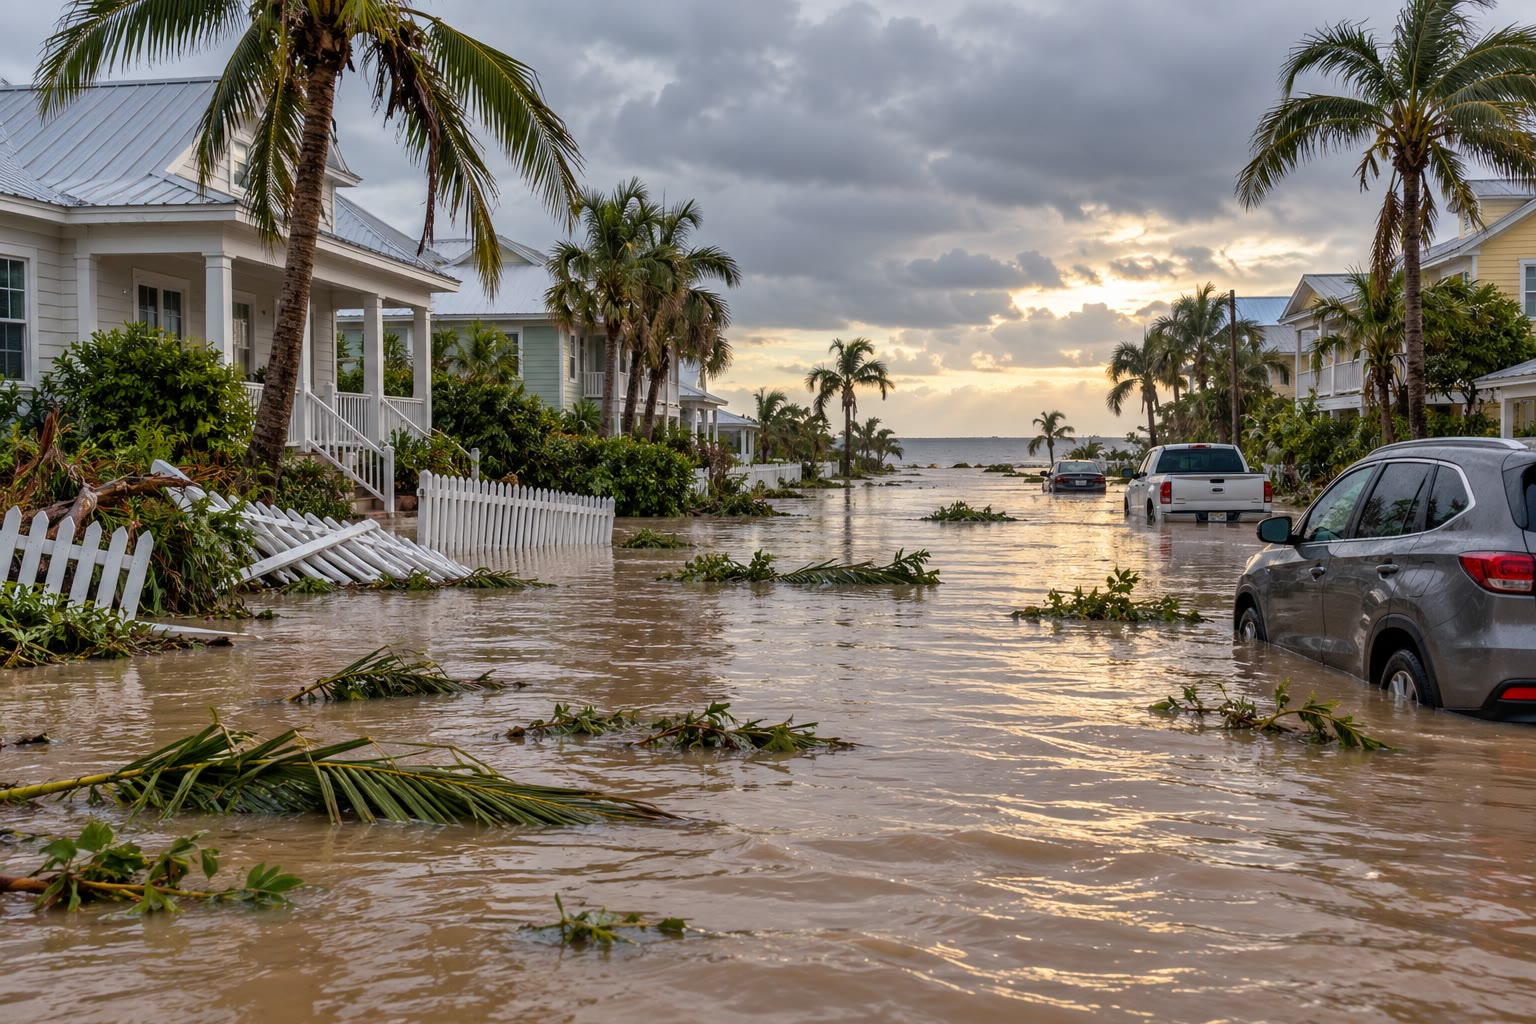
\includegraphics[width=0.7\linewidth]{images/book2/ai/g10-flooded-street.jpg}

{\small Een straat aan de kust op de ochtend na een \omterm{def:g10:storms-and-cyclones:storm-surge}{stormopzet}: zeewater,
geknakte palmen en kapotte hekken.}
\end{omfigure}

\section{Oefeningen}

\begin{exercise}[$\star$]\label{exo:g10:storms-and-cyclones:1}
Definieer een \omterm{def:g10:storms-and-cyclones:thunderstorm}{onweersbui} en \omterm{def:g10:storms-and-cyclones:lightning}{bliksem}. Wat veroorzaakt het geluid van de donder?
\end{exercise}

\begin{exercise}[$\star$]\label{exo:g10:storms-and-cyclones:2}
Definieer een \omterm{def:g10:storms-and-cyclones:tropical-cyclone}{tropische cycloon}, zijn \omterm{def:g10:storms-and-cyclones:tropical-cyclone}{oog} en zijn \omterm{def:g10:storms-and-cyclones:tropical-cyclone}{oogwand}. Waar is de wind het
sterkst?
\end{exercise}

\begin{exercise}[$\star$]\label{exo:g10:storms-and-cyclones:3}
In welke categorie van Saffir--Simpson valt een orkaan met een aanhoudende wind
van \num{70}~knopen? Van \num{120}~knopen? Van \num{140}~knopen? Welke daarvan
zijn zware orkanen?
\end{exercise}

\begin{exercise}[$\star$]\label{exo:g10:storms-and-cyclones:4}
Je telt \num{9} seconden tussen een flits en de donder, en daarna \num{15}
seconden bij de volgende flits. Hoe ver weg was elke flits, en komt het onweer
dichterbij?
\end{exercise}

\begin{exercise}[$\star$]\label{exo:g10:storms-and-cyclones:5}
Leg uit waarom een boom die alleen in een veld staat bij onweer een gevaarlijke
schuilplaats is, en waar je in plaats daarvan naartoe moet.
\end{exercise}

\begin{exercise}[$\star\star$]\label{exo:g10:storms-and-cyclones:6}
Eén knoop is \qty{1852}{m} per uur. Reken \num{64}~knopen en \num{137}~knopen om
naar \unit{m/s} en naar \unit{km/h}.
\end{exercise}

\begin{exercise}[$\star\star$]\label{exo:g10:storms-and-cyclones:7}
Op Aarde zijn er 44 bliksemflitsen per seconde. Hoeveel is dat per dag, en per
jaar?
\end{exercise}

\begin{exercise}[$\star\star$]\label{exo:g10:storms-and-cyclones:8}
Een orkaan heeft een druk in het centrum van \qty{935}{hPa} in een omgeving van
\qty{1010}{hPa}. Hoe hoog is de drukbult van de zee eronder?
\end{exercise}

\begin{exercise}[$\star\star$]\label{exo:g10:storms-and-cyclones:9}
Beschrijf met behulp van de kaart van de banen waar tropische cyclonen ontstaan
en waar ze daarna naartoe gaan. Waarom ontbreken ze op de evenaar zelf?
\end{exercise}

\begin{exercise}[$\star\star$]\label{exo:g10:storms-and-cyclones:10}
De rechte lijn van het druk-winddiagram is $p \approx 1031 - 1.56\,v$
($p$ in \unit{hPa}, $v$ in \unit{m/s}). Welke druk in het centrum geeft ze voor
de ondergrens van categorie 5, \qty{70}{m/s}? Voor een storm van
\qty{40}{m/s}?
\end{exercise}

\begin{exercise}[$\star\star$]\label{exo:g10:storms-and-cyclones:11}
Leg uit waarom een \omterm{def:g10:storms-and-cyclones:tropical-cyclone}{tropische cycloon} snel verzwakt wanneer hij boven land komt,
en waarom hij boven koud water verzwakt.
\end{exercise}

\begin{exercise}[$\star\star\star$]\label{exo:g10:storms-and-cyclones:12}
De geluidssnelheid in lucht is $\sqrt{1.4\,R\,T/M}$, met $R =
\qty{8.314}{J.mol^{-1}.K^{-1}}$, $T$ in kelvin en $M =
\qty{0.02897}{kg/mol}$. Bereken ze bij \qty{0}{\degreeCelsius} en bij
\qty{30}{\degreeCelsius}. Hoeveel verschillen de twee afstanden bij een
vertraging van \qty{9}{s}? Is de regel ``\qty{3}{s} per kilometer'' goed genoeg?
\end{exercise}

\begin{exercise}[$\star\star\star$]\label{exo:g10:storms-and-cyclones:13}
Op een kust wordt een \omterm{def:g10:storms-and-cyclones:storm-surge}{stormopzet} van \qty{4.0}{m} gemeten terwijl een orkaan met
een druk in het centrum van \qty{940}{hPa} (omgeving \qty{1010}{hPa}) aan land
komt. Welk deel van de opzet komt van de drukbult, en welk deel van de wind? Als
hij bij hoogwater aankomt, \qty{1.5}{m} boven gemiddeld zeeniveau, hoe hoog
boven gemiddeld zeeniveau komt het water dan?
\end{exercise}

\begin{exercise}[$\star\star\star$]\label{exo:g10:storms-and-cyclones:14}
Een \omterm{def:g10:storms-and-cyclones:tornado}{tornado} draait met winden van \qty{90}{m/s} op \qty{100}{m} van zijn as;
een orkaan met winden van \qty{60}{m/s} in een \omterm{def:g10:storms-and-cyclones:tropical-cyclone}{oogwand} op \qty{30}{km} van het
centrum. Hoe lang doet de lucht er in elk geval over om één keer rond te gaan?
Vergelijk.
\end{exercise}

\begin{exercise}[$\star\star\star$]\label{exo:g10:storms-and-cyclones:15}
Van de 3\,888 tropische cyclonen van 1980--2024 bereikten er 24 de kracht van
een tropische storm binnen \qty{5}{\degree} van de evenaar, 414 binnen
\qty{10}{\degree}, en 121 voorbij \qty{30}{\degree}. Bereken de drie
percentages. De band binnen \qty{5}{\degree} van de evenaar beslaat ongeveer
\qty{9}{\percent} van het aardoppervlak: wat zou je verwachten als de breedte er
niet toe deed, en wat besluit je?
\end{exercise}

\section{Probleem: de warmtemotor van een orkaan}

\begin{problem}[{Weekendprobleem --- van de regen van één dag tot het vermogen
van de wind}]
\label{pb:g10:storms-and-cyclones:1}
% ledger: aoml:energy, nist:water-latent, earth:Rmean, ipcc:budget-toa (all results computed in figdata/grade-10/cyclones.py or from the rounded data below)
Een gemiddelde orkaan laat per dag \qty{1.5}{cm} regen vallen over een cirkel met
straal \qty{665}{km}. Gebruik een \omterm{def:g10:earth-energy-budget:latent-heat}{latente warmte} van \qty{2.5}{MJ/kg}, een
dichtheid van water van \qty{1000}{kg/m^3}, \qty{86400}{s} in een dag, en het
vermogen van de winden van een gemiddelde orkaan, \qty{1.5e12}{W}.

\medskip
\noindent\textbf{Deel I --- De regen van één dag.}
\begin{enumerate}
  \item Bereken de oppervlakte van de cirkel.
  \item Bereken het volume regen dat er in een dag op valt.
  \item Druk het uit in kubieke kilometer.
  \item Bereken de massa ervan.
\end{enumerate}

\medskip
\noindent\textbf{Deel II --- De vrijgekomen warmte.}
\begin{enumerate}[resume]
  \item Bereken de \omterm{def:g10:earth-energy-budget:latent-heat}{latente warmte} die in een dag vrijkomt bij de condensatie van
        dit water.
  \item Reken die om naar een vermogen.
  \item De hele Aarde absorbeert ongeveer \qty{1.22e17}{W} zonlicht
        (\cref{ch:g10:earth-energy-budget}). Welk deel daarvan maakt één orkaan
        vrij?
  \item Het gemiddelde geabsorbeerde zonlicht is \qty{240}{W/m^2}. Bereken het
        zonlicht dat de oppervlakte van de storm absorbeert, en vergelijk het met
        de \omterm{def:g10:earth-energy-budget:latent-heat}{latente warmte} van de storm.
  \item Wat laat deze vergelijking zien over waar de energie van de storm werd
        verzameld?
\end{enumerate}

\medskip
\noindent\textbf{Deel III --- Waar het water vandaan komt.}
\begin{enumerate}[resume]
  \item Welke massa water moet er elke dag verdampen om deze regen te voeden?
  \item De gemiddelde verdamping van het aardoppervlak voert \qty{82}{W/m^2} af.
        Over welke oppervlakte zou gemiddelde verdamping de \omterm{def:g10:earth-energy-budget:latent-heat}{latente warmte} van de
        storm leveren? Vergelijk met de oppervlakte van de storm.
  \item Vergelijk met de tabel van verzadigingsgehalten uit
        \cref{ch:g10:why-clouds-form} het water dat verzadigde lucht bij
        \qty{28}{\degreeCelsius} en bij \qty{20}{\degreeCelsius} bevat.
  \item Leg uit waarom tropische cyclonen alleen boven warme zeeën ontstaan.
  \item Leg uit waarom ze boven land verzwakken.
\end{enumerate}

\medskip
\noindent\textbf{Deel IV --- De wind.}
\begin{enumerate}[resume]
  \item Bereken de bewegingsenergie die in een dag aan de winden wordt gegeven.
  \item Reken de ondergrens van categorie 3, \num{96}~knopen, om naar
        \unit{m/s} (\num{1}~knoop = \qty{1852}{m/h}).
  \item Lucht vlak boven het zeeoppervlak heeft een dichtheid van ongeveer
        \qty{1.16}{kg/m^3}. Bereken de bewegingsenergie van één kubieke meter
        ervan die met die snelheid beweegt.
  \item Vergelijk de \omterm{def:g10:earth-energy-budget:latent-heat}{latente warmte} die in een dag vrijkomt met de energie van
        de winden in een dag.
  \item Wat gebeurt er met de rest van de vrijgekomen warmte?
  \item Welk deel van de warmte die bij condensatie vrijkomt, wordt wind?
\end{enumerate}
\end{problem}
